  \documentclass[final]{beamer} % beamer 3.10: do NOT use option hyperref={pdfpagelabels=false} !
  %\documentclass[final,hyperref={pdfpagelabels=false}]{beamer} % beamer 3.07: get rid of beamer warnings
  \mode<presentation> {  %% check http://www-i6.informatik.rwth-aachen.de/~dreuw/latexbeamerposter.php for examples
    \usetheme{Berlin}    %% you should define your own theme e.g. for big headlines using your own logos 
   \setbeamercovered{transparent}
  }
  \usepackage[english]{babel}
  \usepackage[latin1]{inputenc}
  \usepackage{amsmath,amsthm, amssymb, latexsym}
\usepackage{tikz}
\usetikzlibrary{arrows}
\usepackage{pgfplots}
\usepackage{fix-cm}
  %\usepackage{times}\usefonttheme{professionalfonts}  % times is obsolete
  \usefonttheme[onlymath]{serif}
  \boldmath
  %\usepackage[orientation=portrait,size=a0,scale=1.4,debug]{beamerposter}                       % e.g. for DIN-A0 poster
  %\usepackage[orientation=portrait,size=a1,scale=1.4,grid,debug]{beamerposter}                  % e.g. for DIN-A1 poster, with optional grid and debug output
  \usepackage[size=custom,width=200,height=160,scale=1.4,debug]{beamerposter}                     % e.g. for custom size poster
  %\usepackage[orientation=portrait,size=a0,scale=1.0,printer=rwth-glossy-uv.df]{beamerposter}   % e.g. for DIN-A0 poster with rwth-glossy-uv printer check
  % ...
  %
  \title[]{{\fontsize{220}{240}\selectfont Clustering and Diagnosing Methods for Rare Genetic Disorders}}
  \author[]{\huge Jialin Song and Jonathan Zung}
  \institute[University of Toronto]{\huge Computational Biology Lab, University of Toronto}
  \date{}
  \begin{document}
  \begin{frame}{}
  \maketitle
  \vspace{-3cm}
    \begin{columns}[T]
      \begin{column}{0.3\linewidth}

     \begin{block}{\Huge Objective}
     \begin{itemize}
    \Large
     \item
     Cluster patients with similar phenotypes
    \item
    Perform diagnoses on patients
     \end{itemize}
      \end{block}

    \begin{block}{\Huge Introduction}
    \Large
    Rare genetic disorders are caused by abnormalities in the human genome. Due to different levels of gene expressions and influences from the environment, even patients with a same underlying disorder may exhibit varying symptoms, which makes accurate diagnoses challenging. By analysing the different amount of information encoded in each phenotype and the structural information provided by ontologies, we can conduct more informative analyses on patients and infer underlying disorders more accurately. 
   \vspace{1cm} 

    \end{block}
    
    \begin{block}{\Huge Resources}
 
    \begin{block}{\Large HPO}
   \begin{columns}[T]
      \begin{column}{.5\textwidth}
      \centering
      \fbox{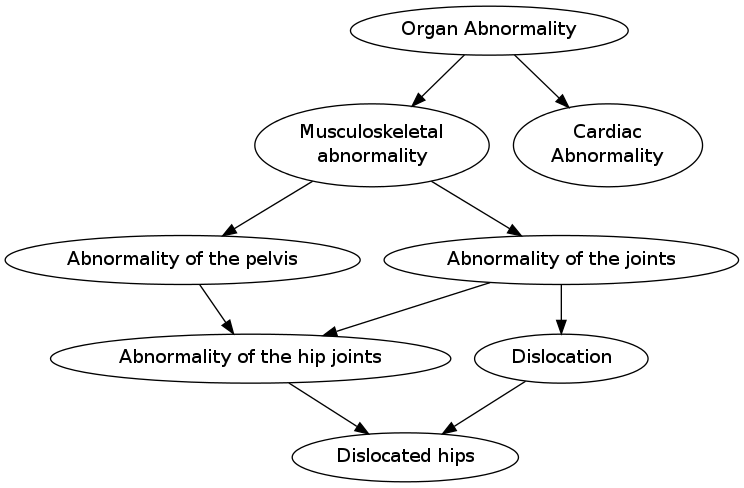
\includegraphics[width = .9\textwidth, , height=25cm]{hpo}}
     \end{column}
     \begin{column}{.5\textwidth}
      \Large
      Human Phenotype Ontology (HPO) organizes standardized terms describing abnormal human phenotypes as a directed acyclic graph. It uses the  {\it{\Large is a}} relation to define parent-child relationships (e.g. a dislocation {\it{\Large is an}} abnormality of the joints).
     \end{column}
   \end{columns}
  \end{block}   

    \begin{block}{\Large OMIM}
      \begin{columns}[T]
        \begin{column}{.5\textwidth}
		\centering
		\vspace{0.5cm}
		\fbox{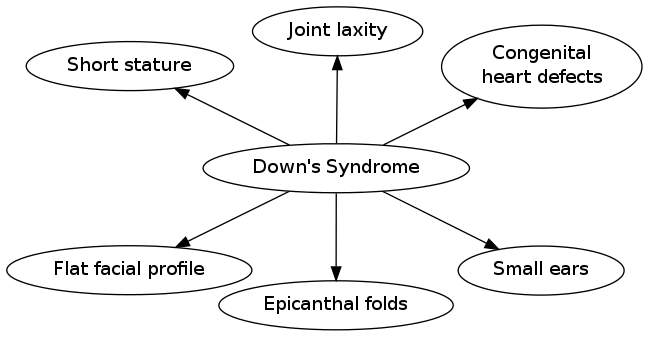
\includegraphics[width = .9\textwidth, height=20cm]{omim_vis}}
        \end{column}
        
        \begin{column}{.5\textwidth}
        \Large
        Online Mendelian Inheritance in Man (OMIM) is a comprehensive collection of human genetic disorders. It associates each disorder with a list of standard human phenotype terms and the probabilities with which they occur given the disorder. For example, it indicates that a patient with Down's syndrome has a probability of 0.5 of having a heart defect.
       \end{column}
    \end{columns}
    \end{block}

  

   \begin{block}{\Large PhenoTips}
      \begin{columns}[T]
        \begin{column} {.5\textwidth}
           \vspace{2.5cm}
           \centering
           \fbox{
\includegraphics[width=.9\textwidth]{PhenoTips}}
        \end{column}
        
        \begin{column}{.5\textwidth}
          \Large
          PhenoTips helps collect phenotype data of patients with genetic disorders using standard HPO terms. Standard terminology helps the process of analysing patients' information by eliminating ambiguities of symptom descriptions.
        \end{column}
      \end{columns}
    \end{block}

   \end{block}

   \begin{block}{\Large Previous Work}
   \Large
   Phenomizer (Robinson et al., 2008 {\it{\Large AM J HUM GENET 83}}, 610 - 615)
   \begin{itemize}
    \item
    Use information content of each HPO term to conduct similarity search
    \item
    For two HPO terms $s, t$, $A(s, t)$ represents their common an-----cestors
    \item
    $p(t) = \frac{\text{\# of associated disorders}}{\text{\# of disorders}}$ for each HPO term $t$
    \item
    $sim(s, t) = \underset{a \in A(s, t)}{max} -\log p(a)$
    \item
    $sim(P,  D)$ = $\frac{1}{2} ( avg[\sum\limits_{s \in P}
    \underset{t \in D}{max} sim(s, t) ]  +  avg[\sum\limits_{t \in D}
    \underset{s \in P}{max} sim(t, s) ]  ) $ 
    \item
    This method can be applied both to measure the similarity between pairs of patients and between patient-disorder pair.
  \end{itemize}
   \end{block}
    \end{column}

    \begin{column}{0.3\linewidth}
     \begin{block}{\Huge Clustering Methods}
     \Large
		\begin{block}{\Large Patient-Patient similarity metrics}
			Define a patient-patient similarity metric, and then apply a standard clustering algorithm (e.g. spectral clustering).

			Examples of similarity metrics:
			\begin{itemize}
				\item Euclidean Metric: Count number of shared traits between two patients.
				\item Information Metric: Essentially, count shared traits weighted by their rarities. Patients sharing rarer traits are more similar.
			\end{itemize}
		\end{block}
		\begin{block}{\Large Mixture Models}
			Formulate a probabilistic model for patient traits with a single latent variable $d$ representing the underlying disorder. Use the EM algorithm to fit the model, then cluster by the inferred values of $d$.

			Examples of mixture models:
			\begin{itemize}
				\item Independent Mixture: Traits are independent given $d$.
				\item Conditional Mixture: Traits are independent given $d$ and their ancestors in HPO.
			\end{itemize}
		\end{block}
     \end{block}
     \vspace{3cm}

     \begin{block}{\Huge Diagnosis Methods}
   
     \begin{block}{\Large Naive Bayes}
     \begin{itemize}
        \Large
    \item
    For a patient $p$, we want to find the disease $d$ with the highest conditional probability $Prob(d \mid p )$
  \vspace{1cm}
  \item
   By Bayes' Theorem: \\
   $Prob(d \mid p) = \frac{Prob(p \mid d) \times Prob(d)}{Prob(p)} \propto Prob(p \mid d) \times Prob(d)$
  \vspace{1cm}
   \item
   Naive Bayes assumes that each phenotype is independent once a disease is given \\
   $Prob(d \mid p) \propto Prob(d) \times \prod Prob(phenotype_i \mid d)$
     \end{itemize}
   \end{block}
    \vspace{1cm}

    \begin{block}{\Large Phenotype Matching}
     \begin{itemize}
     \Large
     \item
     The objective is to measure how close a patient is to the canonical form of a disorder
     \vspace{1cm}
     \item
     For each phenotype of a patient, compute the closest distances to each phenotype annotations of a disease. Construct a distance matrix from the calculated data
     \vspace{1cm}
    \item
    Use the cost matrix to determine the matching between patient's phenotypes and disease annotations that minimizes the total distance
     \vspace{1cm}
    \item
    The minimized distance representing transforming from the real patient to the canonical form of a disorder is used as the measure for closeness
         \end{itemize}
   \vspace{0.5cm}
   \begin{center}
   \fbox{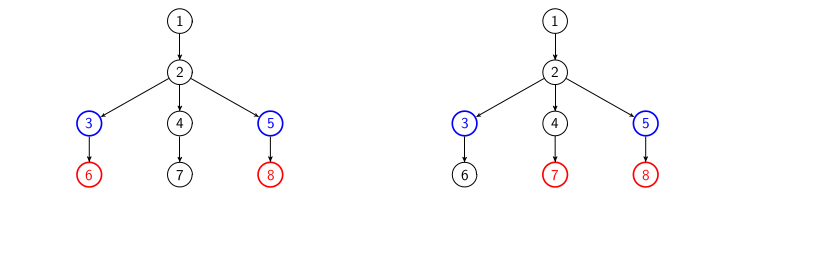
\includegraphics[width=.9\textwidth]{toy_ontology}}
   \\
   \normalsize
   Figure 1: A Toy Ontology Example
   \end{center}
   \begin{columns}[T]
   \begin{column}{.9\textwidth}
   \large
Blue circles are one patient's phenotypes and red ones are annotations of a disorder. In the left one, the real patient can transform into the canonical form of a disorder via $3 \rightarrow 2 \rightarrow 4 \rightarrow 7$ and $5 \rightarrow 8$, resulting in a total cost of 4. While the right one can achieve a total cost of 2 by $3 \rightarrow 6$ and $5 \rightarrow 8$.
   \end{column}
   \end{columns}
   
   \end{block}
  \end{block}

    \end{column}

    \begin{column}{0.3\linewidth}
	\begin{block}{\Huge Datasets}
	\Large
		25 patients from published studies
		\begin{itemize}
			\item 13 with Floating Harbor syndrome
			\item 6 with Rubinstein-Taybi syndrome
			\item 6 with Opitz-Kaveggia syndrome
		\end{itemize}
		1498 simulated patients
		\begin{itemize}
			\item A patient is simulated by selecting a disease at random, and then assigning phenotypes to the patient according to the probabilities recorded on OMIM. Noise is then added by appending some of the 100 most common traits and then performing a random walk on the HPO graph. 
		\end{itemize}
	\end{block}
    \begin{block}{\Huge Results}
    \begin{block}{\Large Clustering Results }
      \centering
\fbox{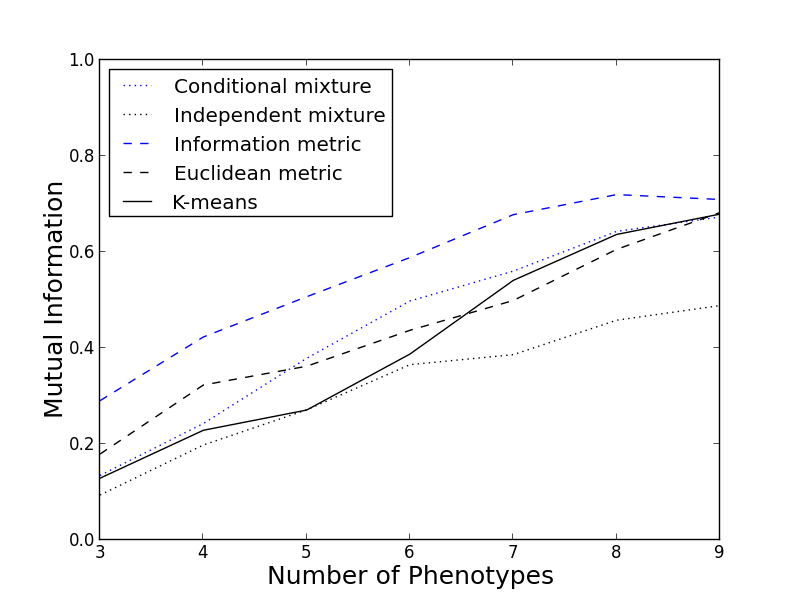
\includegraphics[width=0.7\textwidth]{cluster_comparison.png}} \\
   Figure 2: Comparison of Clustering Methods
    \end{block}

    \begin{block}{\Large Diagnosis Results}

\centering {
\fbox{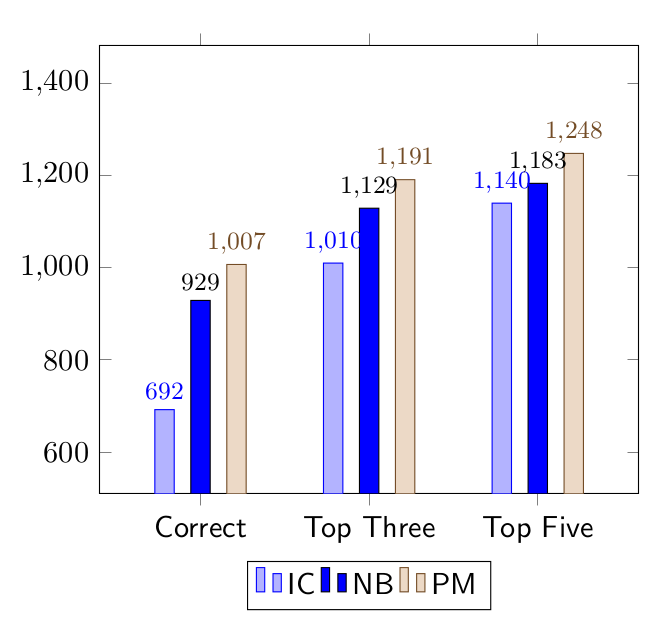
\includegraphics[width=.7\textwidth ]{sim_patients}}
   \\
   Figure 3: Diagnosis Results for 1498 Simulated Patients  \\}
   \vspace{0.5cm}
   \begin{columns}
   \begin{column}{.7\textwidth}
   \large
   Naive Bayes made near 35\% more correct diagnoses than Phenomizer by utilizing frequency data of abnormal phenotypes, while phenotype matching outperformed naive Bayes by utilizing structural information in HPO. 
  \end{column}
  \end{columns}

      \end{block}
    \end{block}
    \end{column}
    \end{columns}
  \end{frame}
  \end{document}
